\documentclass[12pt]{article}
\usepackage[utf8]{inputenc}
\usepackage[margin=1in]{geometry}
\usepackage{indentfirst}
\usepackage{amsmath}
\usepackage{bm}
\usepackage[euler]{textgreek}
\usepackage{float}
\usepackage{newfloat}
\usepackage{graphicx}
\usepackage{caption}
\usepackage{subcaption}
\usepackage{textcomp}
\usepackage{mathptmx}

\DeclareCaptionFont{10pt}{\fontsize{10pt}{12pt}\selectfont}
\captionsetup{justification=raggedright, singlelinecheck=false, font=10pt}
\captionsetup[figure]{labelfont={bf},labelsep=period}
\captionsetup[table]{labelfont={bf},labelsep=period}
\DeclareFloatingEnvironment[name={Table}]{tabfloat}

\title{%
Observations and implications of artificial vegetation on suspended sediment capture in laboratory flume experiments \\
\bigskip
\large 2018-19 Undergraduate Honors Thesis \\
\large Department of Geography \\
\large University of California, Berkeley \\
Advisor: Laurel Larsen}
\author{Justin Nghiem}
\date{}

\begin{document}

\maketitle

\begin{abstract}
    Sediment transport and storage are increasingly significant processes in wetlands because of the rising rate of coastal land loss. Vegetation has the ability to augment sediment retention in wetlands by physically trapping particles. As a result, understanding interactions of vegetation and sediment transport has valuable implications for wetland morphodynamics especially under climate changes. In particular, predictive models of particle capture have considerable practical application. We hypothesize that the introduction of vegetation stem density and surface type parameters to current models improves predictive accuracy of effective capture efficiency, defined as the probability that a transported particle adheres to a vegetation stem, because these properties encode perturbations that impose controls on effective capture efficiency. We ran laboratory experiments in a recirculating flume with an array of greased wooden dowels, which modeled emergent biofilm-covered vegetation stems, to test this hypothesis and to perform an independent study of the influence of artificial vegetation on sediment capture. Two treatments, a control experiment without dowels and an experiment with dowels, were performed. An exponential model was fitted from which particle capture rates for the treatments were estimated and compared. The presence of dowels led to a larger particle capture rate compared to the particle capture rate of the treatment without dowels, supporting the notion that wetland vegetation stands enhance sediment retention. Furthermore, dowel interactions with flow produced an order-of-magnitude reduction in the particle capture rate due to gravitational settling. We found that, among existing models of effective capture efficiency, a model with a similar vegetation stem density and surface setting compared to the conditions in this study provided the best prediction of the calculated effective capture efficiency of the dowel treatment. This finding supported the hypothesis that additional dependencies on vegetation stem density and surface in models of effective capture efficiency may improve prediction accuracy.
\end{abstract}

\pagebreak

\section{Introduction}

Sediment transport to coastal regions has wide consequences for key processes like land progradation, water quality, and ecological productivity. With the prospect of climate change and sea level rise looming, the significance of sediment load to coastal lands has grown considerably. Britsch and Dunbar [1993] found that an estimated 17.8\% of land in a study area in the Louisiana Coastal Plain had been lost from the 1930s to 1990, with a maximum rate of land loss of about 42 mi\textsuperscript{2} per year in 1974. This trend will be compounded in the near future as rates of relative sea level rise increase. The combination of erosion and land subsidence along the coast threatens not only its physical characteristics, but also its dense human environment and infrastructure. Coastal and deltaic zones are home to a large human population worldwide, on the order of hundreds of millions, and represent a rich social and economic network [Syvitski et al., 2009].

Improved understanding of sediment retention and transport through river deltas will be instrumental in answering these long-standing questions. Analytic solutions for particle capture are well-defined at the extremes of creeping and potential flow conditions but are poorly characterized in transitional regions typical in wetlands, thus necessitating experimental work and the fitting of empirical models. In particular, past studies have explored the interactions between sediment particles and vegetation in flumes with vegetation features representative of wetlands and have found that the presence of vegetation in sediment-laden flows may enhance sediment retention by promoting deposition and direct adherence to vegetation stems [Fauria et al., 2015; Wu et al., 2011; Palmer et al., 2004]. Previous workers have estimated predictive models for particle capture, which are valuable tools for forecasting wetland morphology [Palmer et al., 2004; Fauria et al., 2015].

Drawing on this work, we propose that vegetation stem density and stem surface are necessary parameters for more accurate predictive models of effective capture efficiency in natural wetland flow conditions with emergent vegetation because they integrate scales of interactions between particles and stems. Vegetation stem density records the number of vegetation stems per area. Stem surface describes the type of surface of the vegetation collector, such as smooth, greased, or biofilm-covered. Stem density may significantly impact particle capture, and hence effective capture efficiency, because it contains information on potential effects of the presence of multiple stems, such as in the case of interference due to wake generation in the flow downstream of the stems. Stem surface may be important for particle capture because the stem surface microscale may dictate whether or not a particle is able to adhere to the stem. For example, roughness elements on a surface may facilitate particle trapping.

We hypothesize that effective capture efficiency models may improve prediction accuracy through the inclusion of vegetation stem density and surface inputs. As a corollary, existing empirical models, estimated with specific vegetation conditions, would more accurately predict effective capture efficiency for a setting with similar vegetation conditions. We test this similarity argument using new laboratory flume experiments. In this study, these experiments were performed to validate models of effective capture efficiency and to independently infer the influence of vegetation on removal of suspended sediment from transport in wetland flows. Two treatments in a recirculating flume were tested, one in which wooden dowels were installed to mimic wetland vegetation and one without dowels as an experiment control. A fixed sediment mass was added at the start of each experiment, and suspended sediment mass concentration was recorded over time.

This study contributes to further understanding of sediment routing in wetlands by testing the influence of a large vegetation array at a higher water depth of 40 cm. Previous studies have not examined water depths above 17 cm despite the observation that water depth in wetlands usually ranges up to 50 cm [Kadlec, 1990]. More concretely, the results of the experiments in this study, and future experimental and theoretical work, may inform wetland management to maximize sediment retention and mitigate land loss.

\section{Methods}

\subsection{Physical Setting}

The removal of sediment in suspended load has been theorized as consisting of the particle capture mechanisms of (1) \textit{direct interception} in which objects in the flow trap particles directly, (2) \textit{inertial impaction} in which particles with sufficiently large inertia deviate from flow lines and impact onto objects that trap them, (3) \textit{gravitational deposition} in which particles settle on the stream bed, and (4) \textit{diffusional deposition} in which particles impact and are trapped on objects due to random motions [Rubenstein and Koehl, 1977; Spielman, 1977].

The collector Reynolds number $Re_c$ defines the flow conditions and structure for flow through emergent vegetation, in which the vegetation stems are ``collectors" that capture sediment particles as flows are transmitted through vegetation. In particular, $Re_c$ is defined as

\begin{equation} \label{Rec}
    Re_c=\frac{u d_c}{\nu}
\end{equation}

\noindent where $u$ is the flow velocity, $d_c$ is the collector diameter, and $\nu$ is the fluid kinematic viscosity. At creeping flows ($Re_c < 1$) and potential flows ($Re_c > 1000$), analytic equations readily describe particle capture due to direct interception [Fuchs, 1964]. However, intermediate $Re_c$ are more characteristic of wetlands in which transitional flows tend to dominate but do not have an analytic expression, hence the need to perform more physical tests and better validate empirical predictive models with laboratory experiments.

\subsection{Background Theory}

\subsubsection{Sediment Transport Model}

The relationship of suspended particles transported in a flow and the collectors in the flow (e.g. vegetation stems) may be modeled with probabilities of particle-collector interaction and particle retention on the collector. The capture efficiency $\eta$ is defined as the ratio of particle diameter and collector diameter [Palmer et al., 2004; Fauria et al., 2015]. The capture efficiency may be written as

\begin{equation} \label{ce}
    \eta=\frac{b}{d_c}=P(\text{interaction with collector})
\end{equation}

\noindent where $b$ is the upstream width of flow transporting the particles that is undisturbed by the presence of the collector and $d_c$ is the collector diameter (Figure \ref{fig_capeff}).

\begin{figure}[H]
    \centering
    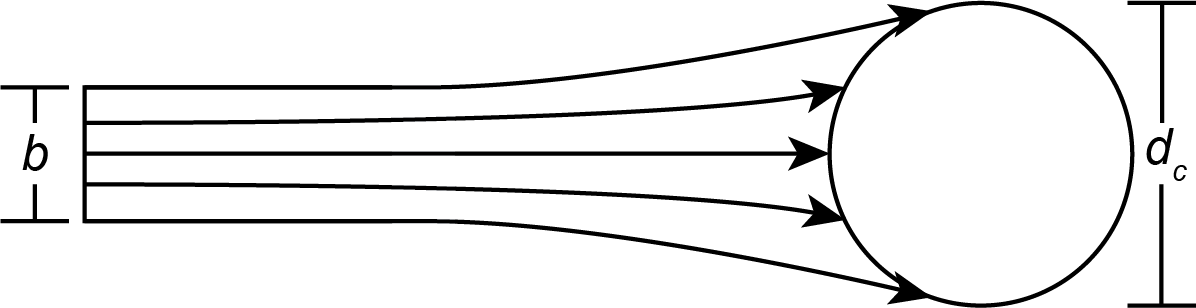
\includegraphics[width=6.5in]{capture_efficiency.png}
    \caption{Illustration of particle capture efficiency. $b$ is the upstream width of flow. $d_c$ is the collector diameter. After Figure 1 in Palmer et al. [2004].}
    \label{fig_capeff}
\end{figure}

However, this formulation is solely a function of flow conditions and does not account for whether or not particles are retained on the collector. The effective capture efficiency $\eta^\prime$ rectifies this shortcoming by introducing an additional factor for the probability that the collector surface traps and retains a particle that makes contact with the collector [Fauria et al., 2015]. The effective capture efficiency $\eta^\prime$ has the form

\begin{equation} \label{effcapeff1}
    \eta^\prime=p_r \frac{b}{d_c}=P(\text{retention} \mid \text{interaction}) P(\text{interaction with collector})
\end{equation}

\noindent in which $p_r$ is the probability of the collector retaining the particle given that the particle collides with the collector. By this definition, the effective particle efficiency quantifies the overall rate at which collectors remove particles from the suspended load.

In order to quantify changes in sediment concentration with time, a first-order relationship between these variables must be obtained. Fauria et al. [2015] described the reduction in suspended sediment concentration with time as an exponential decay, combining an advection-diffusion equation and the Rouse equation for suspended sediment profiles. This equation has the form

\begin{equation} \label{expmod}
    \phi(t)=\phi_0 e^{-kt}
\end{equation}

\noindent where $\phi$ is the sediment concentration at some reference height above the bed as a function of time, $\phi_0$ is the initial sediment concentration at the reference height, $k$ is the particle capture rate (s\textsuperscript{-1}), and $t$ is time (s). The sediment concentrations may be volumetric or mass concentrations. For the purposes of this study, sediment concentrations were in units g/L or, equivalently, kg/m\textsuperscript{3}. This equation implies that the particle capture rate may be estimated given measurements of sediment concentration with time at a reference height above the bed.

Additionally, Fauria et al. [2015] showed that the particle capture rate $k$ may be written as

\begin{equation} \label{addk}
    k=k_s+k_c
\end{equation}

\noindent where $k_s$ is the particle capture rate attributable to gravitational settling of particles and $k_c$ is the particle capture rate attributable to particle retention on collectors. This relation is valuable for separating the influence of vegetation collectors from gravitational deposition on the particle capture rate. Moreover, $k_c$ and effective capture efficiency $\eta^\prime$ are related, under further considerations of the Rouse equation and an advection-diffusion description of suspended sediment concentration, by the equation

\begin{equation} \label{effcapeff2}
    \eta^\prime=\frac{k_c}{u d_c l_c}
\end{equation}

\noindent where $u$ is the flow velocity (m/s) and $l_c$ is the collector length per unit volume (m/m\textsuperscript{3}) [Fauria et al., 2015]. In equation \ref{effcapeff2}, $k_c$ depended on the specific experiment treatment while the other terms were constant known experiment parameters.

\subsubsection{Stress Model}

The law of the wall and the Shields criterion were used to characterize the stress and sediment transport regimes in the flume. The equation for the law of the wall is

\begin{equation} \label{ltw}
    u(z)=\frac{1}{\kappa} u_* \log{\frac{z}{z_0}}
\end{equation}

\noindent where $u$ is the flow velocity as a function of elevation $z$ from the bed (m/s), $\kappa$ is the dimensionless von Kármán constant (taken to be 0.4), $u_*$ is the shear velocity (m/s), $z$ is the elevation from the bed (m), $\log$ denotes the natural logarithm, and $z_0$ is a characteristic length of bed roughness (m). The law of the wall assumes a turbulent flow regime, a requirement that is likely fulfilled from the Reynolds number (see Flume Description). The statement of the law of the wall is useful because it quantifies the bed shear stress, through the shear velocity, once the flow velocity at a known height is measured.

Knowledge of the bed shear stress may then be applied in the Shields criterion for the initiation of particle motion from the bed. The Shields criterion defines an empirical relationship between the particle Reynolds number, in which particle diameter is the characteristic length, and the dimensionless critical shear stress at which a particle on the bed begins to move,

\begin{equation} \label{shields}
    \tau_*=\frac{\tau_b}{(\rho_s-\rho_w)gD}
\end{equation}

\noindent where $\tau_b$ is the bed shear stress, $\rho_s$ is the sediment density, $\rho_w$ is the fluid density (water in this case), $g$ is gravitational acceleration, and $D$ is particle diameter [García, 2008]. The relationship between particle Reynolds number and $\tau_*$ was estimated using an approximate mathematical relation [Brownlie, 1981]. The combination of the law of the wall and Shields criterion provided a quantitative description of stress regimes and consequent sediment transport modes in the flume experiments.

\subsection{Experimental Design}

The goal of this study was to examine the influence of artificial vegetation on suspended particle capture in wetland environments. Two treatments were designed and performed to address this question. In all treatments, a fixed quantity of sediment was added to the flume and recirculated in flow conditions similar to those of wetlands, and the change in sediment mass concentration with time was recorded over a period of 100 min. In the first treatment, water and sediment circulated through the flume without any obstructions in the flow. In the second treatment, wooden dowels, which were coated with silicone grease and extended through the water column, were added to simulate the presence of emergent biofilm-covered vegetation stems. Detailed descriptions of each part of the experimental design follow in the remainder of this subsection.

\subsubsection{Flume Description}

\begin{figure}[H]
    \centering
    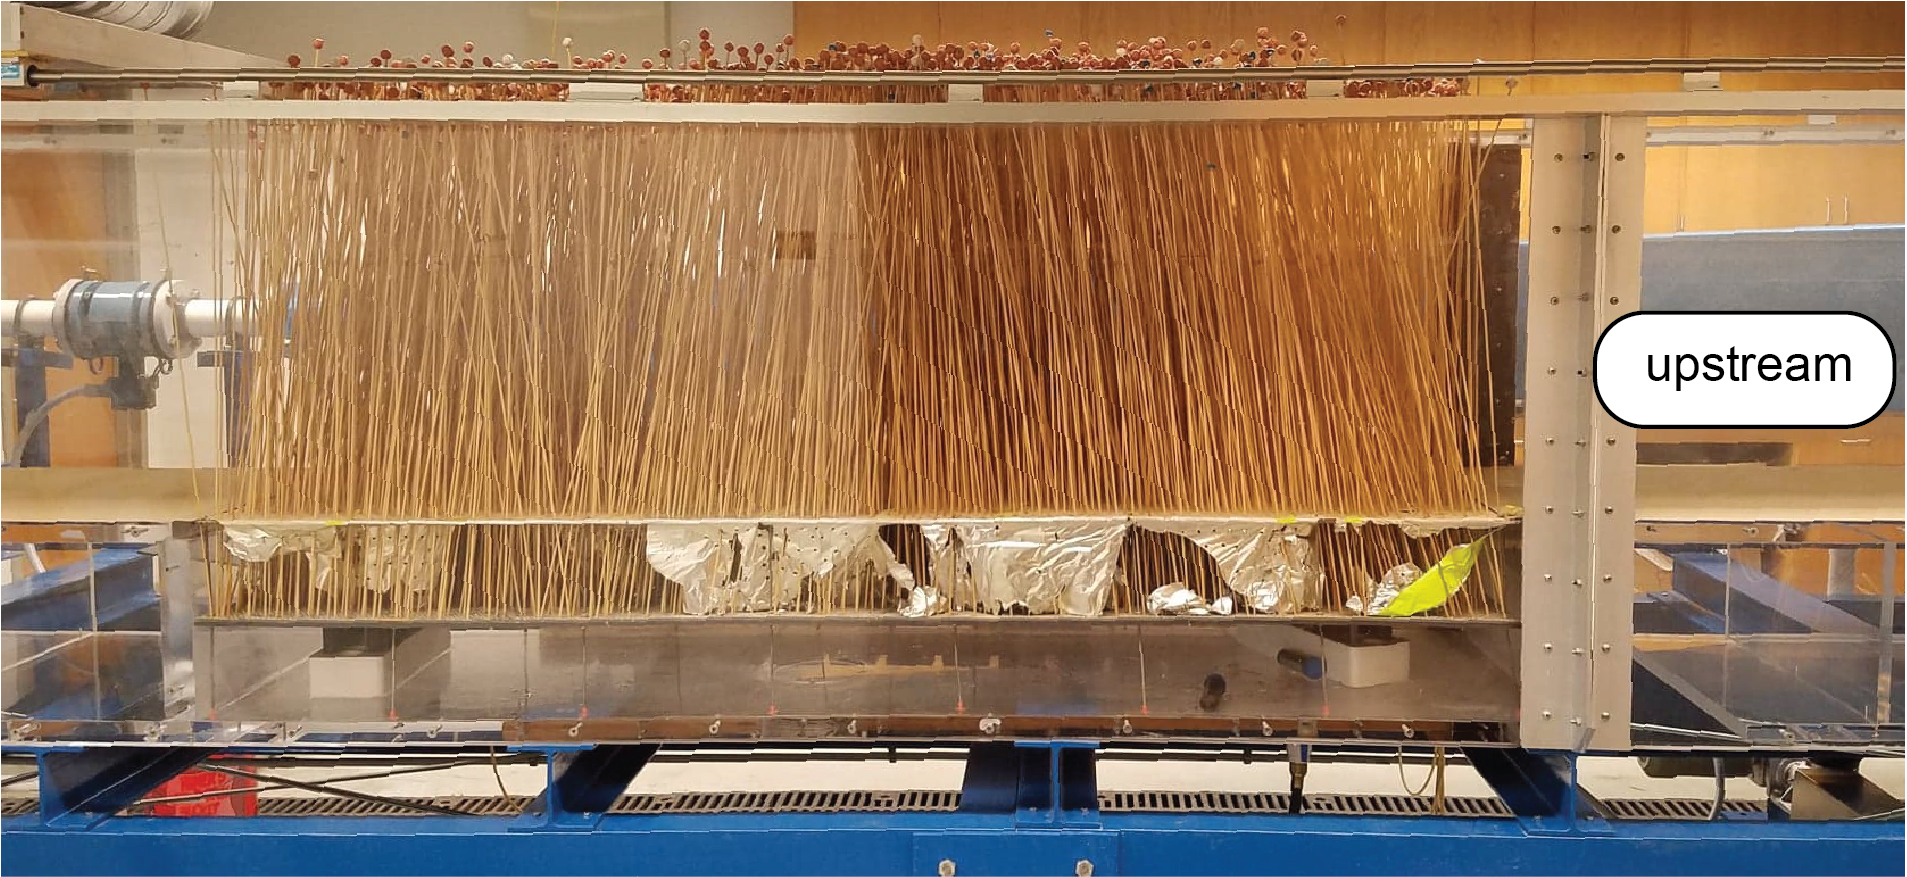
\includegraphics[width=6.5in]{flume_photos.png}
    \caption{Side profile of the recirculating flume used in this study. The open channel portion is pictured, with the dowels installed in the test section. The covered region is behind the open channel in this figure. The foil is visibly torn beneath the top of the PVC sheet because of dowel installation (see Artificial Vegetation Preparation for more details).}
    \label{fig_flumephoto}
\end{figure}

The laboratory experiments were performed in the ecogeomorphology recirculating flume in McCone Hall, Berkeley, CA. The flume consisted of an open channel (length 5.25 m, width 0.6 m, height up to 0.45 m) and a covered region with a pump to route water from the downstream end back to the upstream inlet. The flume was outfitted with a single stage, close-coupled disc pump in which parallel rotating discs draw in fluid in parallel layers using viscous drag [Discflo]. According to the manufacturer, a stationary boundary layer along the pump walls ensures that the transmitted flow is laminar, meaning sediment is minimally disrupted as it passes through the pump. The flume had an approximate maximum capacity of 3.1 m\textsuperscript{3} when filled to the maximum water depth of 0.45 m. In addition, the open channel portion of the flume had a removable false bed with the dimensions 0.6 m across the channel and 1.95 m along the channel (area 1.17 m\textsuperscript{2}).

For all experiments in this study, the flume was operated with a water depth of 0.40 m in the open channel segment, translating to an approximate flume water volume of 2.9 m\textsuperscript{3}. The pump was set such that the average discharge of the flume was 0.0136 m\textsuperscript{3}/s and the average flow velocity in the open channel portion was approximately 0.057 m/s. This flow velocity reflects moderate natural flow conditions in wetlands and is within the ranges of velocities examined in previous studies [Palmer et al., 2004; Fauria et al., 2015]. The Reynolds number for a bare flume under these conditions, taking the characteristic length scale to be the water depth, was approximately $2.2 \times 10^4$, indicating a transitional flow between turbulent and laminar regimes. Holding these flow conditions constant, the experiment treatments differed solely on the presence or absence of dowels simulating natural vegetation stems.

\subsubsection{Artificial Vegetation Preparation}

In order to model the presence of vegetation in the flow, wooden dowels were installed in the false bed portion of the flume (hereafter referred to as the ``test section"). Individual dowels had an approximate diameter of $\frac{1}{8}$ in. Dowels were placed upright in the test section through a perforated PVC sheet flush with the bed elevation upstream and downstream of the test section. The PVC sheet had regularly-spaced holes (diameter 0.1875 in) in a staggered pattern, with a spacing of 0.313 in between the centers of any two adjacent holes. Before placing the PVC sheet in the flume, the PVC sheet was wrapped in aluminum foil to limit flows between the above and below bed regions through holes unoccupied by dowels. The dowels were additionally coated with a thin uniform layer of silicone grease to mimic biofilm, then installed in the test section by puncturing through the foil into the holes in the PVC sheet. The resulting dowel array modeled a stand of emergent vegetation stems with a roughly uniform biofilm surface.

The structure of the PVC sheet allowed for a maximum dowel density, defined as the number of dowels per area, of approximately 18,200 dowels/m\textsuperscript{2} (e.g. every hole occupied). The dowel density was directly equivalent to the vegetation stem density. For the treatment with dowels, the dowel density was approximately 1,450 dowels/m\textsuperscript{2} with the dowels placed in a uniform staggered pattern throughout the test section. The dowels were long enough such that they were emergent, extending from the flume bed up past the water surface. Small clay balls were added to the tops of all dowels to prevent the otherwise buoyant dowels from floating out of place. For the treatment without dowels, no dowels were installed in the test section so the test section had a bed surface of aluminum foil over the PVC sheet.

\begin{table}[H]
    \caption{Experiment settings and parameters}
    \begin{subtable}{1\textwidth}
        \caption{Summary of key experiment settings for all treatments. The only variable is the presence or absence of dowels in the test section. All numeric values are averages across the relevant spatial scale.}
        \label{tab_experimentsettings}
        \centering
        \begin{tabular}{c c c c}
            \textbf{Treatment} & \textbf{Flow velocity} (cm/s) & \textbf{Dowel density} (m\textsuperscript{-2}) & \textbf{Sediment mass added} (g) \\
            \hline
            1 & 5.7 & 0 & 200 \\
            \hline
            2 & 5.7 & 1450 & 200 \\
            \hline
        \end{tabular}
    \end{subtable}
    \newline
    \vspace*{0.1 in}
    \newline
    \begin{subtable}{1\textwidth}
        \caption{Additional dowel parameters for treatment 2. Frontal area/volume is the frontal area of dowels in a cross-section in the test section normalized by test section volume. Dimensionless dowel density is the dowel density scaled by the square of dowel diameter. Solid volume fraction is proportion of test section volume occupied by dowels.}
        \label{tab_dowelparameters}
        \centering
        \begin{tabular}{c c c}
            \textbf{Frontal area/volume} (m\textsuperscript{2}/m\textsuperscript{3}) & \textbf{Dimensionless dowel density} & \textbf{Solid volume fraction} (\%) \\
            \hline
            4.604 & 0.01462 & 1.148 \\
            \hline
        \end{tabular}
    \end{subtable}
\end{table}

\subsubsection{Sediment Preparation}

The sediment used for the experiments was crushed walnut shell (WF-5 200 mesh walnut shell flour) [Composition Materials]. The crushed walnut shell had a specific gravity of approximately 1.3, and so was slightly denser than water [Composition Materials]. The manufacturer sieve analysis showed that 100\% of the walnut shell passes through a no. 60 sieve (250 \textmu m sieve opening) and 88\% passes through a no. 200 sieve (74 \textmu m sieve opening).

The particle size distribution of crushed walnut shell diameters was directly measured using a laser diffraction instrument (Sequoia Scientific LISST-Portable\textbar XR). The instrument analyzed approximately 10 mg of crushed walnut shell suspended in 100 mL of water, using a mixer to agitate the sample in the instrument and ensure adequate sampling. Using a Fraunhofer diffraction optical model, volumetric concentrations in particle size bins from 0.34 to 500 \textmu m were measured. The concentrations were normalized to obtain an empirical probability density function (PDF) of walnut shell particle diameters. A corresponding cumulative density function (CDF) was constructed using the same data.

At the start of each experiment, the sediment was introduced into the upstream section of the open channel with a dispensing jug over approximately 3 minutes. A mass of 200 g crushed walnut shell was well-mixed in about 4 gal of water in the jug before adding to the flume in each experiment. Previous tests with the flume showed that water recirculated back to the same point, under the given flow settings, in about 3 minutes. Thus, sediment addition using the dispensing jug ensured an approximately uniform initial sediment concentration throughout the flume.

\subsection{Instruments}

In order to record necessary variables during the experiment, three instruments were used: (1) an acoustic Doppler velocimeter (ADV) to measure local flow velocities, (2) a pair of peristaltic pumps to measure sediment mass concentrations over time, and (3) a set of sediment traps to measure particle settling in the test section.

\subsubsection{Acoustic Doppler velocimeter}

The ADV infers flow velocity at a point in three dimensions by using the Doppler effect to transform the change in pitch of a transmitted pulse as it is reflected by particles traveling in the flow into a flow velocity [Nortek]. As a result, the ADV relies on the assumption that particle velocity matches flow velocity. The ADV also features a temperature probe, which was used to measure the average water temperature.

During the experiments, the ADV was mounted in the upstream portion of the open channel, about 1 m upstream from the edge of the test section in the center of the flow with the probe at 20 cm from the bed (Figure \ref{fig_flumeschematic}). The ADV collected data throughout each experiment. Outside of the actual experiment runs, additional data were collected using the ADV in the flume with the same dowel structure as the dowel treatment in this study. These data were the input for the bed shear stress estimate and analysis with the Shields criterion. Since the same dowel arrangement was in place for these extra measurements, the flow field was expected to be representative of the flow field during the experiment.

\subsubsection{Peristaltic Pump Sampling}

A pair of peristaltic pumps was installed to collect water samples from the flume along the open channel (Figure \ref{fig_flumeschematic}). Each pump was connected to three hoses, which were routed to three sampling elevations in the flume (5, 14, and 27 cm from the bed) in the center of the flow. The opening of each hose in the flume was oriented pointing directly opposite and parallel to the direction of flow along the flume to maximize the representativeness of each water sample. This pump structure was placed at two locations in the flume, one immediately upstream of the test section and the other immediately downstream of the test section. In sum, there were six distinct sampling sites in the flume (5 cm from the bed upstream of the test section, 14 cm upstream, 27 cm upstream, 5 cm downstream, 14 cm downstream, and 27 cm downstream).

Throughout each experiment, the peristaltic pumps continuously drained water from each of the sampling sites described at a flow rate of approximately 50 mL/min per hose. Water samples were collected for each sampling site at 5-minute intervals for the duration of each experiment (100 min). All water samples were collected in clean plastic bottles, which were typically filled to their capacity of around 140 mL. The relatively low flow rate, combined with the addition of water when the sediment was introduced, implied that the net change in water volume in the flume during an experiment was negligible.

\subsubsection{Sediment Traps}

Sediment traps were installed at nine well-spaced locations in the PVC sheet in the test section to collect samples of settled particles during the experiments (Figure \ref{fig_traps}). Sediment traps were fabricated from cylindrical plastic syringe tubes with an approximate diameter of 2.5 cm. The syringe bottoms were replaced with perforated PVC, creating a depth of approximately 3.8 cm between the sediment trap opening and bottom. Before each experiment, each sediment trap was lined at the bottom with glass microfiber filter paper and installed in the test section such that the sediment trap opening was effectively flush with the bed of the test section. During each experiment, particles settled into the sediment traps and collected on the filter paper. The perforated bottoms of the sediment traps were designed to better capture the amount of settled mass than a closed design, which would have required particles to displace water out of the sediment trap and would have underestimated the settled mass as a result. The relatively small diameter and modest number of sediment traps also limited any unforeseen mixing between the flow in the open channel and the reservoir below the surface of the test section that would have occurred with larger openings or more sample points.

During the experiment with dowels, one of the sediment traps failed resulting in only eight sediment trap data points for that experiment. The failed sediment trap was disregarded in all subsequent steps. The necessary calculations were performed with the eight remaining sediment traps.

\begin{figure}[H]
    \centering
    \caption{Flume Instrument Diagrams}
    \begin{subfigure}{1\textwidth}
        \centering
        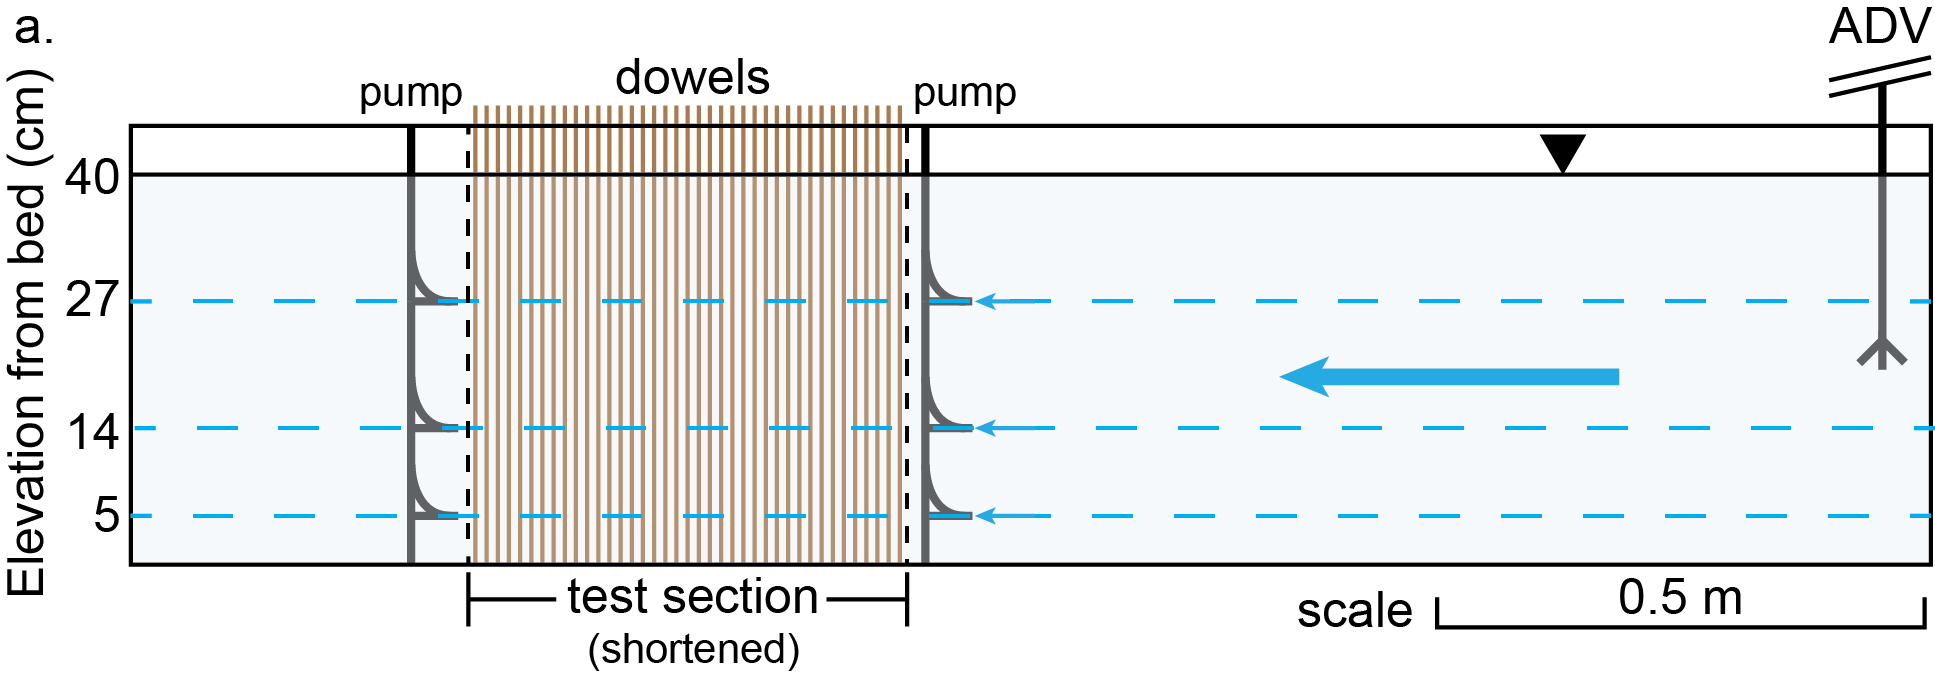
\includegraphics[width=6.5in]{flume_side_schematic.png}
        \caption{Schematic side profile of open channel portion for the dowel treatment. The uppermost 1.2 m in the upstream reach, lowermost 0.7 m in the downstream reach, and a 1.5-m stretch of the test section have been excluded from the view for clarity. All lengths are otherwise to scale. Peristaltic pumps and ADV were positioned in the center of the flume width.}
        \label{fig_flumeschematic}
    \end{subfigure}
    \begin{subfigure}{1\textwidth}
        \centering
        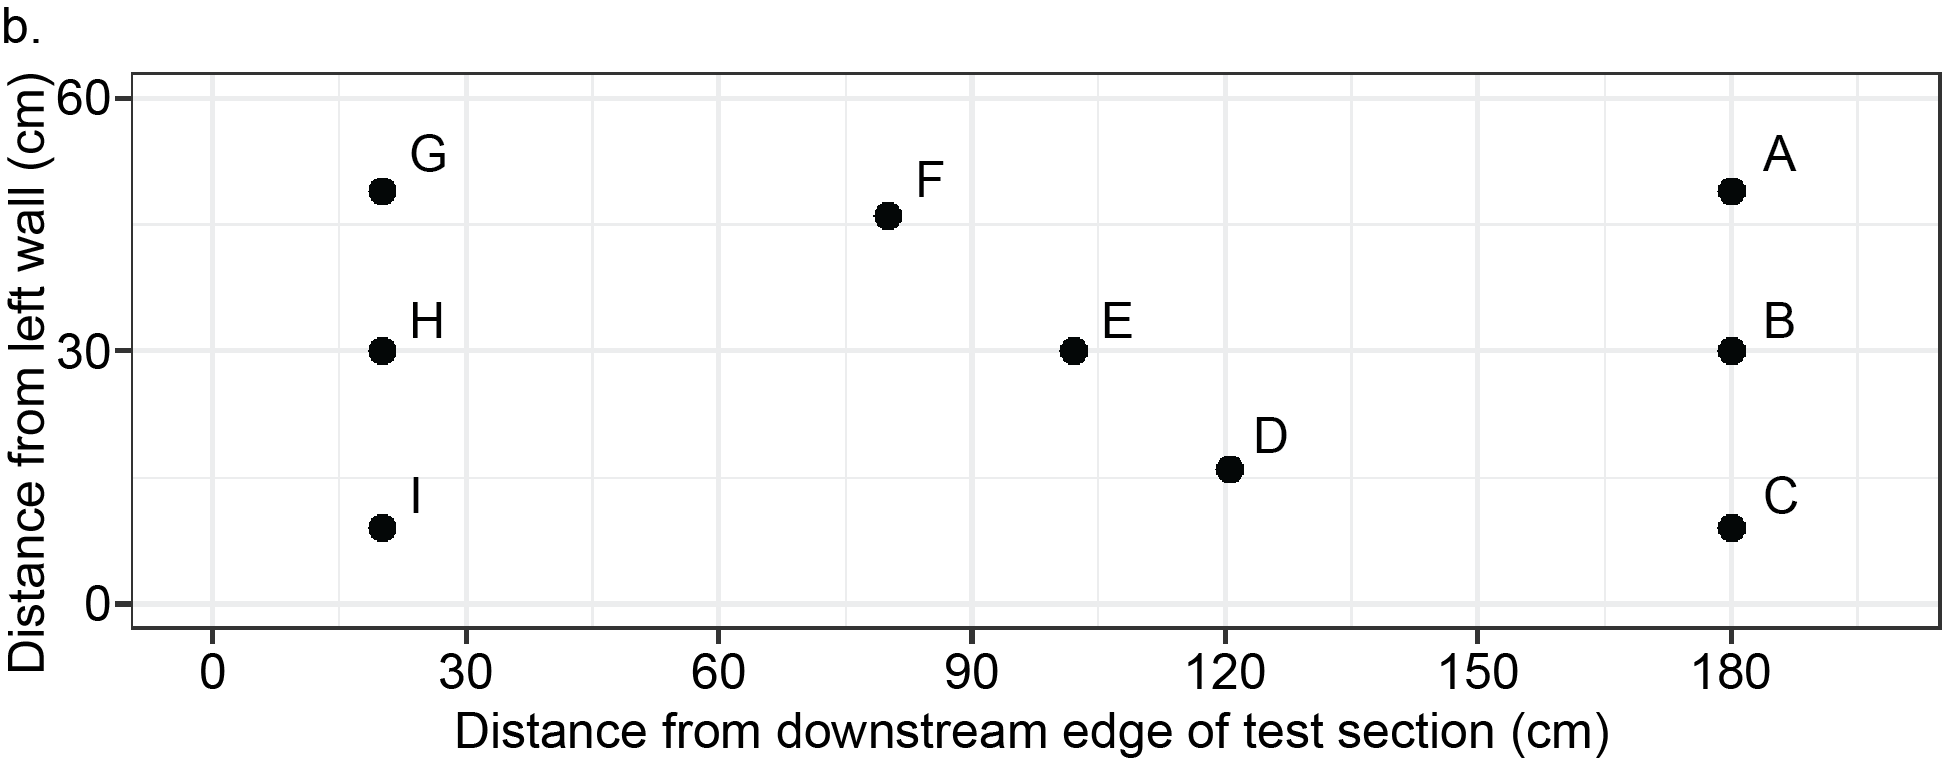
\includegraphics[width=6.5in]{flume_ts_schematic.png}
        \caption{Overhead view of sediment trap positions in the test section labeled by identification letter. Sediment trap I (bottom left) failed during the dowel experiment and was excluded from data analysis. The test section was 1.95 m long and 0.6 m wide. The flow direction was from right to left. Lengths are to scale. Sediment trap areas are not to scale.}
        \label{fig_traps}
    \end{subfigure}
\end{figure}

\subsection{Filtering Protocol}

After each experiment, the water samples from the peristaltic pumps were processed using a standard filtering protocol. Glass microfiber filter papers were heated in an oven at 40\textdegree C at least overnight to remove residual moisture. Each filter paper was weighed after heating. Next, all water samples were filtered using a vacuum pump through the glass microfiber filter papers. The filter papers were returned to the oven to remove excess moisture and re-weighed. The difference between the post-filtration mass and the pre-filtration mass of the filter paper was taken to be the collected sediment mass in a sample. The mass concentration of each sample was calculated to be this mass divided by the sample’s measured water volume. The result was a time series of mass concentration for all combinations of sampling height and upstream/downstream location.

\subsection{Statistical Methods}

Statistical methods were used for model fitting of and inference on the mass concentration time series. First, the Wilcoxon signed rank test was used to evaluate the statistical significance of the differences in mass concentration across upstream and downstream samples. Each pair was taken to be the samples with identical sampling height and time point, only differing in upstream/downstream location.

Second, the results of the inference informed the parameter estimation procedure for the suspended sediment exponential model of equation \ref{expmod}. In the two experiments, upstream and downstream pump sampling locations were indistinguishable in terms of sediment concentration (see Treatment Comparison for more details). As a result, all data were pooled and used to fit the model parameters for each experiment. The initial concentration $\phi_0$ and particle capture rate $k$ were estimated using ordinary least squares (OLS) regression on the equation

\begin{equation} \label{logconc}
    \log{\phi}=\log{\phi_0}-kt
\end{equation}

\noindent in which $\log$ denotes the natural logarithm and the transformed quantities $\log{\phi_0}$ and $-k$ were the explicitly estimated parameters.

\subsection{Separating the effects of settling and capture on collectors}

For the treatment with dowels, the individual contributions of settling and capture on collectors were estimated using mathematical considerations of the background theory and measurements of settling from sediment trap data. The particle capture rate $k$ may be partitioned into a rate related to gravitational settling ($k_s$) and a rate related to interaction and capture of particles on collectors ($k_c$), as seen from equation \ref{addk}.

An equation is derived here to solve for $k_s$ and $k_c$ using a combination of known and estimated parameters in the experiments. The total mass settled throughout the flume during the experiment ($m_s$) is given by the integral

\begin{equation} \label{ms_integral}
    m_s=\int_0^T k_s m_0 e^{-kt} \ \text{d}t
\end{equation}

\noindent where $m_0$ is the initial mass added to the flume and $T$ is the length of time of the experiment. The initial mass times the exponential term models the overall decline in sediment mass over time due to gravitational deposition and capture on dowels, following equation \ref{expmod} with the exception that mass has been substituted in place of concentration. This expression for the sediment mass in the flow at a given time is multiplied by the capture rate constant due to settling ($k_s$) to give the instantaneous downward sediment mass flux. Then, the expression is time-integrated to yield the total mass settled on the flume bed over the course of the experiment.

The integral may be evaluated and the result rearranged to solve for the unknown $k_s$, which has the form

\begin{equation} \label{ks_solved}
    k_s=\frac{m_s k}{m_0 (1-e^{-kT})}
\end{equation}

\noindent in which all quantities on the right-hand side of the equation may be estimated from experiment data. The combined particle capture rate $k$ was estimated using mass concentration data from filtered water samples collected via the peristaltic pumps. The initial sediment added $m_0$ and the total time $T$ of the experiment were recorded for each run. In all experiments in this study, the initial mass was approximately 200 g and the experiment duration was approximately 6000 s.

Finally, the total mass settled in the flume during an experiment $m_s$ was estimated using two data sources to account for different regimes of settling in the flume. First, spatial thin-plate spline interpolation of sediment trap data was used to quantify settling in the test section in which the dowels were expected to influence the pattern and intensity of settling compared to an empty test section. Second, the simple average of the settled masses recorded by the sediment traps in a run without dowels was scaled by area to estimate the amount of sediment settled in the dowel-free open channel regions outside of the test section in the run with dowels. It was assumed that no settling occurred outside of the open channel portion of the flume, a choice that was justified because smaller cross-sectional area elevated flow velocity in the regions outside of the open channel.

Once $k_s$ was calculated for the dowel treatment, $k_c$ could then be calculated as simply $k_c=k-k_s$ because of the partition of $k$ in equation \ref{addk}.

\subsection{Comparison with Predictive Models}

The estimated effective capture efficiency from the dowel run was compared against predictions from two models to test model accuracy and suitability. In particular, calculated effective capture efficiency was compared to two empirical models, one from Palmer et al. [2004] and one from Fauria et al. [2015]. Palmer et al. [2004], using experiments of a single cylindrical collector in a flow with both smooth and rough silicone-greased surfaces, found that

\begin{equation} \label{palmer}
    \eta^\prime=0.224 Re_c^{0.718} R^{2.08}
\end{equation}

\noindent where $Re_c$ is the collector Reynolds number and $R$ is the ratio of particle diameter and collector diameter. Fauria et al. [2015] found that, for the stem density $7209 \ \text{m}^{-2}$ and presence of biofilm in flume experiments using emergent plastic grass blades to model vegetation,

\begin{equation} \label{fauria}
    \eta^\prime=2.06 Re_c^{-1.14} R^{0.65}
\end{equation}

\noindent in which the variables are defined identically as in the Palmer et al. [2004] model. The parameters $Re_c$ and $R$ for the dowel experiment were used to compute the predicted effective capture efficiency from the two models. Since particle diameters spanned a range of values, the predicted effective capture efficiency given a model was calculated by an average of predicted effective capture efficiencies weighted by the proportion of the particle size distribution contained in discrete particle size bins.

\section{Results}

\subsection{Particle Diameter Distribution}

The particle diameter distribution of the crushed walnut shell was measured with a laser diffraction instrument (Figure \ref{fig_sizedistn}). The empirical PDF indicated a roughly symmetric distribution in logarithmic space, with a peak of approximately 32.55 \textmu m. The bulk of the particles ranged from 1 to 200 \textmu m in diameter, an interval that contained approximately 95\% of the particle distribution and so was considered to be the effective particle diameter range. From the estimated CDF, the median grain diameter ($D_{50}$) was approximately 25.20 \textmu m and the grain diameter exceeding 84\% of the size distribution ($D_{84}$) was approximately 57.53 \textmu m.

The laser diffraction results for particle diameter distribution were in approximate agreement with the manufacturer sieve analysis by visual inspection of the measured CDF plotted with the sieve analysis data points, an observation that supported the measurement validity (Figure \ref{fig_sizedistn}). The empirical CDF overestimated the proportion of the particle diameter distribution smaller than 74 \textmu m compared to the sieve analysis result at the same diameter. However, this discrepancy was relatively small and could be attributable to slight variability between the representative samples used in the sieve analysis and in the laser diffraction method used here.

\begin{figure}[H]
    \centering
    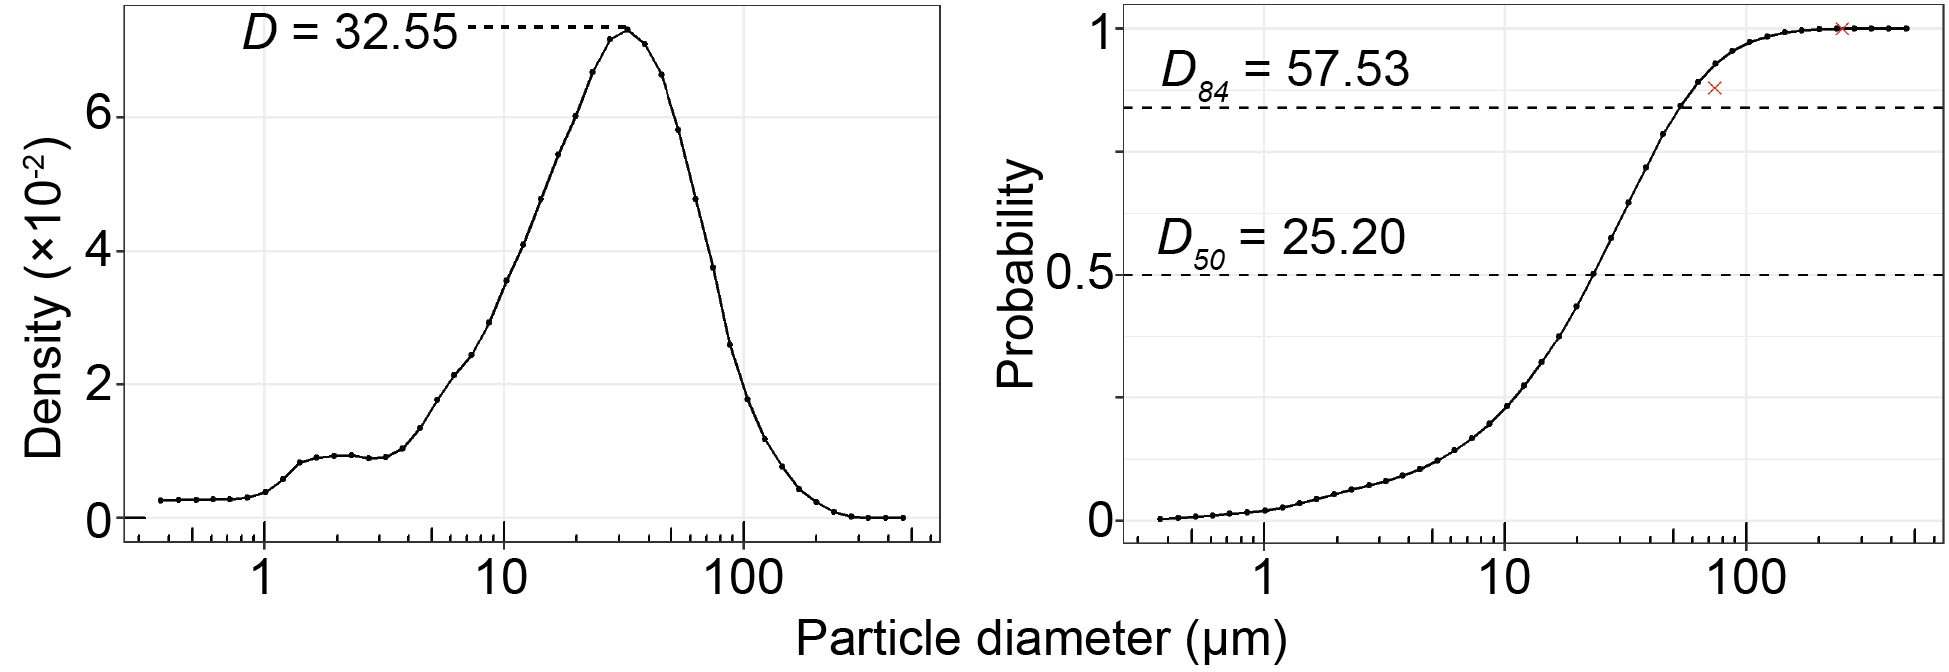
\includegraphics[width=6.5in]{size_distn.png}
    \caption{Left: Walnut shell particle diameter PDF. The peak in the distribution occurs at a particle diameter of 32.55 \textmu m. \\
    Right: Walnut shell particle diameter CDF. The horizontal dashed lines mark the $D_{50}$ (median) and $D_{84}$ particle diameters. The two cross marks indicate the manufacturer sieve analysis data points.}
    \label{fig_sizedistn}
\end{figure}

\subsection{Stress Conditions}

The stress conditions were computed for two locations in the flume. The first location was 1 m upstream from the edge of the test section in the center of the flow, which was taken to be representative of regions of steady flow without the influence of dowels. The second location was well within the interior of the test section in the presence of dowels in the center of the flow, which was taken to be representative of the test section in dowel treatment in which dowels interacted with the flow.

The shear velocities at these two locations were estimated using the law of the wall and the average of ADV readings of the local flow velocity at a height of 10 cm from the flume bed. In the calculations, the characteristic bed roughness length $z_0$ was taken as 57.53 \textmu m, which was the $D_{84}$ grain diameter obtained from the particle diameter distribution. Additionally, the values for the density and kinematic viscosity of water were assumed for a water temperature of 20\textdegree C, which was the approximate average water temperature measurement from the ADV.

\begin{table}[H]
    \centering
    \caption{Estimated shear-related parameters from the law of the wall and the Shields criterion. The listed diameters were the threshold maximum diameters of particles that would begin to move by fluid force at the given shear stress. The error bounds were the twice the sample standard deviation of measurements at a given location.}
    \label{tab_shear}
    \begin{tabular}{c c c c}
        \textbf{Region} & \textbf{Shear velocity} & \textbf{Bed shear stress} & \textbf{Particle diameter} \\
         & ($\times 10^{-3}$ m/s) & ($\times 10^{-3}$ Pa) & (\textmu m) \\
        \hline
        Upstream, no dowels & $3.078 \pm 0.198$ & $9.456 \pm 0.0197$ & 8.28 \\
        \hline
        Test section, dowels & $2.937 \pm 1.278$ & $8.611 \pm 0.816$ & 7.18 \\
        \hline
    \end{tabular}
\end{table}

The similarity in estimated shear parameters indicated that the presence of dowels had a minimal effect on transport conditions (Table \ref{tab_shear}). In the upstream region without dowels, the estimated shear velocity was $3.078 \times 10^{-3}$ m/s, translating to an approximate bed shear stress of $9.456 \times 10^{-3}$ Pa. Under this stress, the critical particle diameter for initial motion was estimated as 8.28 \textmu m. In the test section with dowels, estimates of $2.937 \times 10^{-3}$ m/s for shear velocity, $8.611 \times 10^{-3}$ Pa for shear stress, and 7.18 \textmu m for critical particle diameter were calculated. The error bounds, which were computed from twice the standard deviation of continuous flow velocity measurements at given locations, indicated that the shear velocities and bed shear stresses were within the range of being indistinguishable from each other by location, supporting the notion that dowels had a negligible influence on shear stress conditions at the resolution of the ADV.

\begin{figure}[H]
    \centering
    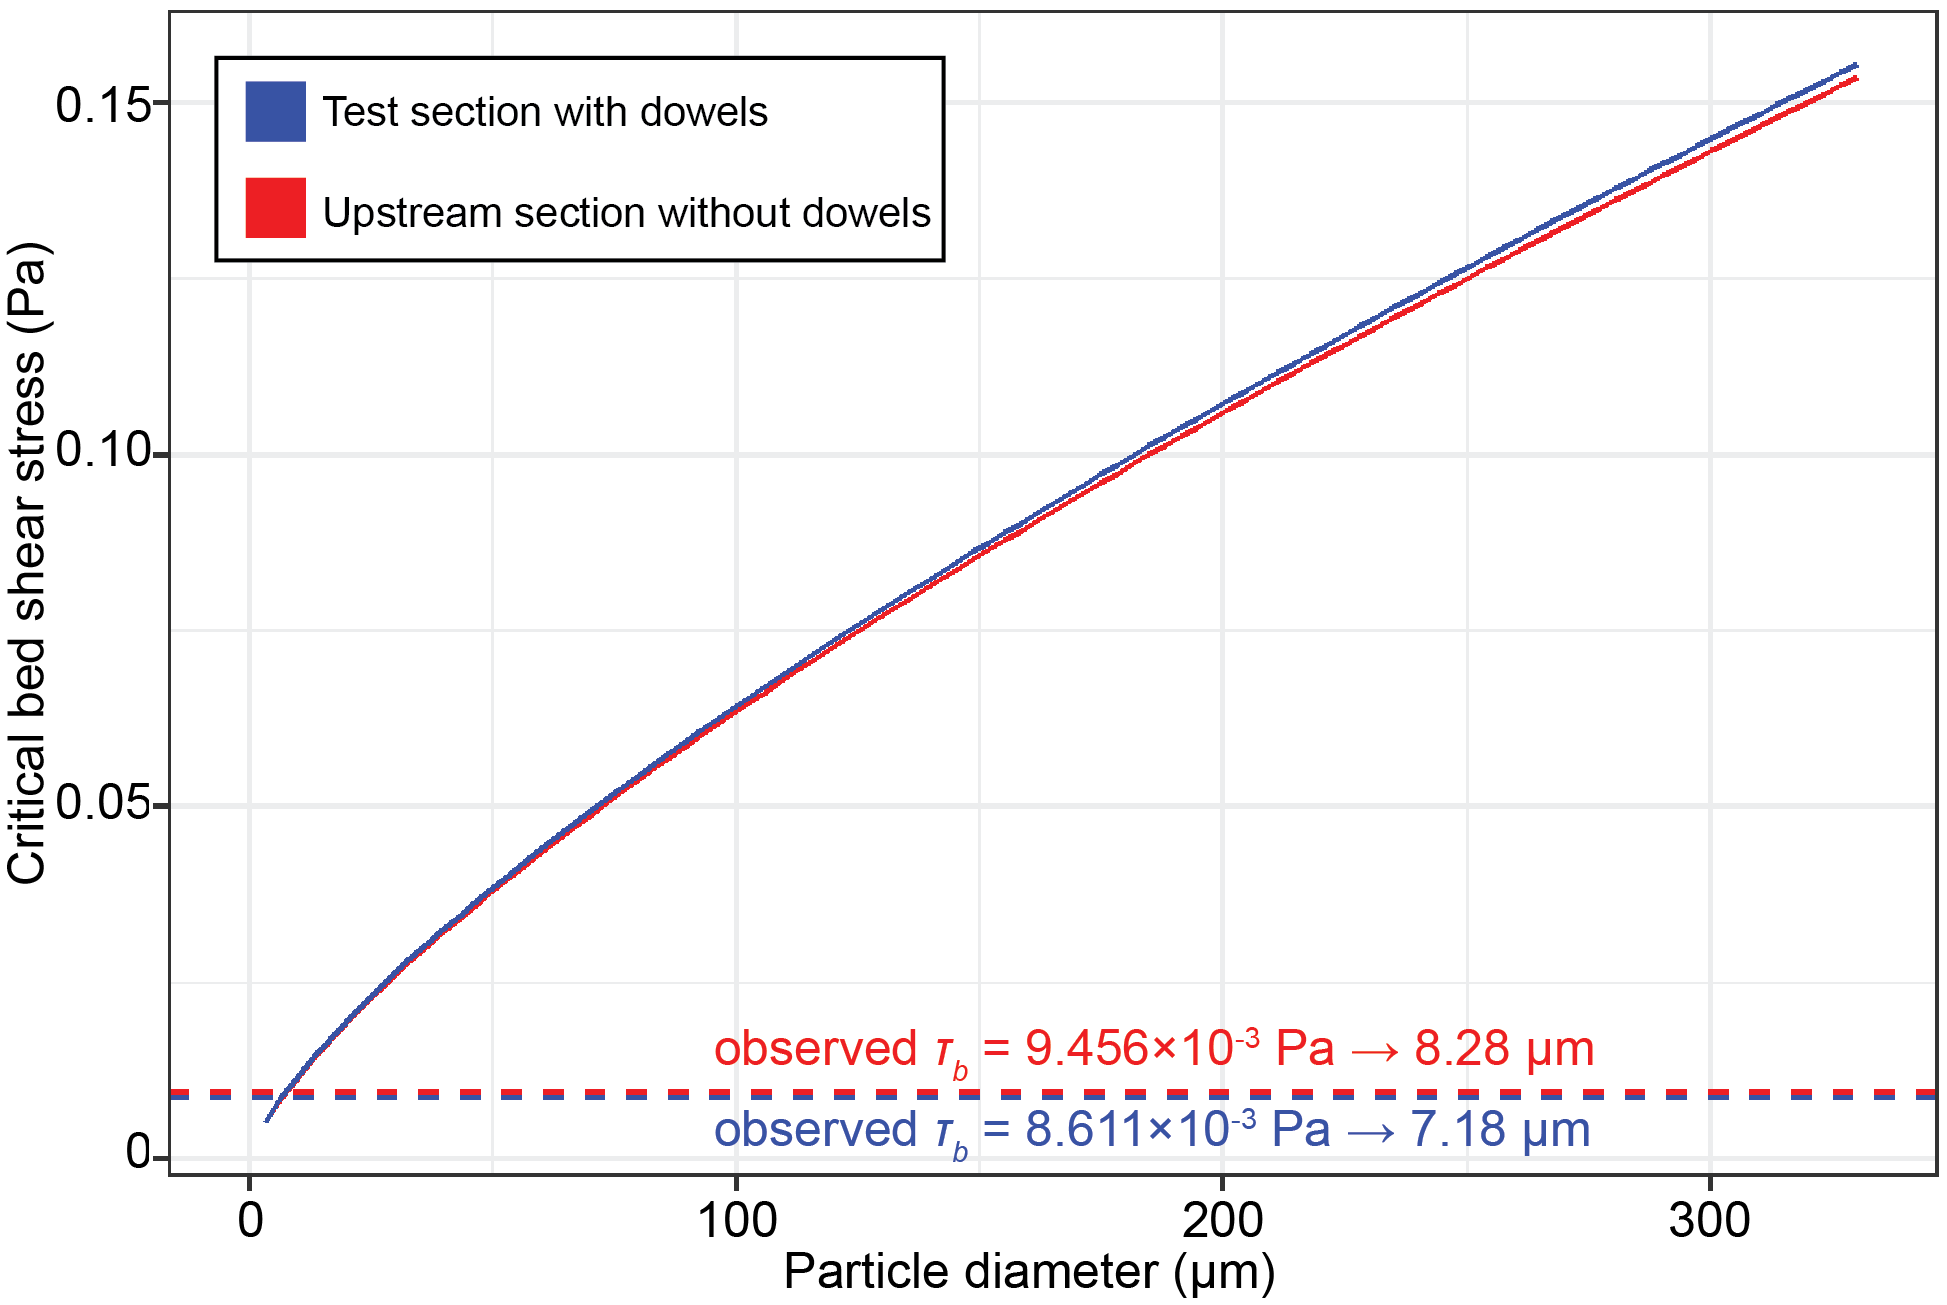
\includegraphics{shields.png}
    \caption{Critical bed shear stress for initial particle motion as a function of particle diameter from 0 to 330 \textmu m. The dashed lines mark the observed bed shear stress and the corresponding particle diameter for each of the two regions.}
    \label{fig_shields}
\end{figure}

The Shields criterion was applied to infer a general transport description for the range of walnut shell particle sizes. Using the Shields criterion, the critical bed shear stress for initial particle motion as a function of particle diameter (0 to 330 \textmu m) was enumerated (Figure \ref{fig_shields}).

In general, the relationship of particle diameter and critical stress was again similar across locations indicating that dowels had a marginal effect on the mode of sediment transport. The observed bed shear stress was only large enough to initiate motion from the bed of particles up to about 8 \textmu m (hereafter called the ``critical diameter"). Based on the particle diameter distribution, this critical diameter exceeded the diameters of approximately 18.88\% of the particle distribution. Thus, although a majority of particles were larger than this critical particle diameter, a substantial portion of particles were subject to incipient motion on the bed at the estimated bed shear stress.

This analysis revealed that once particles with diameters larger than the critical diameter of approximately 8 \textmu m had settled on the bed, very little resuspension occurred because the particles were too large to be moved by the shear stresses in the flume regardless of the presence of dowels. In addition, these magnitudes of remobilization for these particles were conservative because shear velocity was measured in the center of flow where shear velocity tends to be maximized due to reduced wall drag.

However, particles with diameters smaller than the critical diameter, consisting about 18.88\% of the sediment sample, may have remobilized into suspended load or bed load once settled on the bed. Despite this potential particle re-entrainment, the Stokes’ law settling velocity at the critical diameter was calculated as $1.12 \times 10^{-5}$ m/s, leading to a total vertical downward displacement of about 0.07 m over the 6000-second duration of an experiment. It may be inferred that particles with diameters smaller than the critical diameter did not have a sufficiently large settling velocity to reach the bed from top of the water column, which was the point at which the sediment was added. Thus, this fraction of the particles traveled as suspended load throughout an experiment. As an important note, the ideal conditions for Stokes’ law were not satisfied in the flume, but still provided a valid order-of-magnitude upper bound on settling velocity. Settling velocity goes as the square of particle diameter, so particles with diameters smaller than the critical diameter had settling velocities that were far smaller than the Stokes’ settling velocity of the critical diameter. In addition, turbulent mixing in the flume would tend to reduce settling velocities.

With these findings, the sediment transport setting of the experiments may be described as a declining suspended load over time with little evidence for appreciable bed load or resuspension. According to the Shields analysis, this transport regime occurred because particles large enough to settle on the bed during the experiment were too large to be moved as bed load by the fluid force. Particles that could be set in motion by the fluid force once settled on the bed had settling velocities that were too small for them to reach the bed during an experiment. These results supported application of the suspended particle model of equation \ref{expmod} to the experiment data by ensuring that the peristaltic pump sampling method was measuring purely suspended particle concentrations and not bed load (e.g. through saltating particles).

An additional test lent further evidence for the absence of resuspension. In the test, the flume was operated at the same flow conditions without dowels as in this study after all sediment from a previous run had settled on the bed. Negligible concentrations were recorded at the heights sampled by the peristaltic pumps suggesting that particles small enough for incipient motion tended to travel along the bed, if they moved at all. This test supported the lack of resuspension in the flume at the settings used in this study, even in the case in which particles with diameters smaller than the critical diameter had settled on the bed. The subsequent analysis focused on the rate of change of the suspended load in the presence or absence of the dowel vegetation proxies.

\subsection{Treatment Comparison}

\begin{table}[H]
    \centering
    \caption{Estimated treatment parameters with uncertainty bounds equal to twice the corresponding standard error.}
    \label{tab_estimates}
    \begin{tabular}{c c c c}
        \textbf{Treatment} & $\boldsymbol{\phi_0}$ (g/L) & $\boldsymbol{k}$ ($\times 10^{-4} \ \text{s}^{-1}$) & $\boldsymbol{Re_c}$ \\
        \hline
        1 (no dowels) & $49.80 \pm 2.02$ & $1.620 \pm 0.0601$ & NA \\
        \hline
        2 (dowels) & $51.55 \pm 2.03$ & $2.229 \pm 0.0924$ & 180.6 \\
        \hline
    \end{tabular}
\end{table}

The treatment with dowels had, compared to the treatment without dowels, a faster decline in sediment mass concentration over the length of an experiment (Figure \ref{fig_timeseries}). Accordingly, the estimated particle capture rate $k$ for the dowel treatment was $2.229 \times 10^{-4} \text{s}^{-1}$ ($R^2=0.9603$) which was greater than that for the no dowel treatment at $1.620 \times 10^{-4} \text{s}^{-1}$ ($R^2=0.9506$; Table \ref{tab_estimates}). These differences in the particle capture rates between runs were distinguishable as evidenced by the relatively tight uncertainty bounds, obtained from the model fit, which did not overlap (Table \ref{tab_estimates}). In contrast, the initial concentrations were well within bounds of each other and thus indistinguishable as expected because an identical sediment mass was added at the start of each run. The high coefficients of determination for both treatments supported the validity of the theoretical exponential model for suspended load. The collector Reynolds number $Re_c$ was approximately 180.6 for the dowel treatment and indicated a transitional flow.

Aligning with the conclusion drawn from the comparison of particle capture rates, the dowel treatment had a visibly faster decline in sediment mass concentration as observed in the time series plot (Figure \ref{fig_timeseries}). From a more physically meaningful perspective, the time-averaged difference in concentration between the treatments in the final 10 minutes of the experiments (5400 to 6000 s) was 5.31 g/L, found by integrating the exponential models.

\begin{figure}[H]
    \centering
    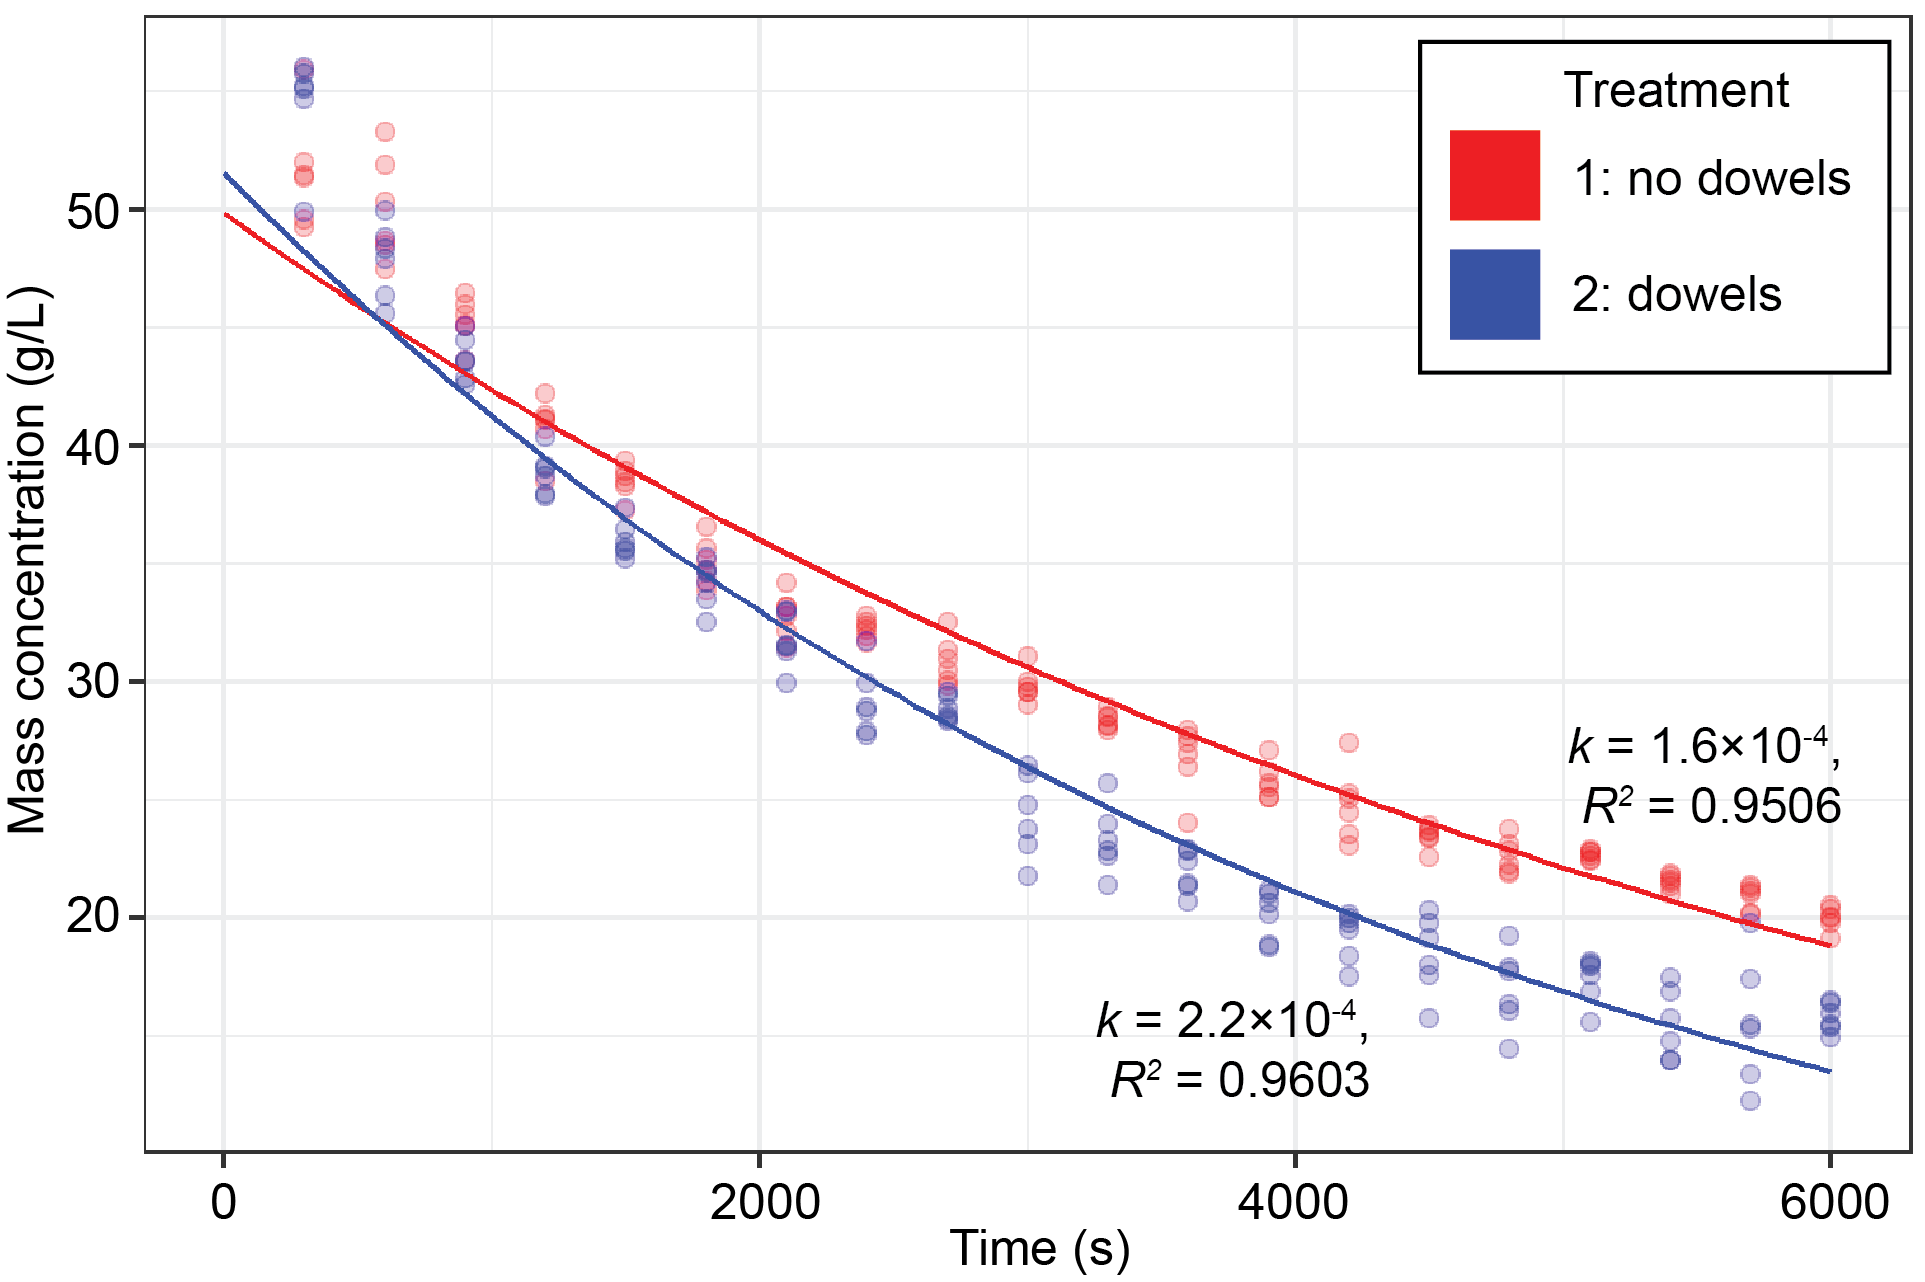
\includegraphics[width=6.5in]{timeseries.png}
    \caption{Time series of sediment mass concentration for the two treatments. The points do not distinguish between sampling height and longitudinal flume location.}
    \label{fig_timeseries}
\end{figure}

The treatment results showed an appreciable difference in particle capture rates. However, an additional question for the dowel treatment was whether there was a significant difference in mass concentrations between the upstream and downstream sampling sites. Theoretically, the presence of the dowels in the test section would enhance particle removal so the upstream concentration should be consistently larger than the downstream concentration for the same time point. The mean of the paired differences of the upstream and downstream concentrations for the dowel treatment was 0.274 g/L, indicating that the upstream concentration was slightly larger on average as expected.

The nonparametric Wilcoxon signed rank test was used to evaluate the significance of this difference. The null hypothesis was that the difference was equal to 0 (indistinguishable upstream and downstream concentrations). The one-sided alternative hypothesis was that the difference was greater than 0 (upstream concentration larger than downstream concentration). The test produced a $p$-value of 0.336, meaning that there was little evidence in the data to support the claim that the upstream concentration was significantly larger than the downstream concentration at the 0.05 significance level.

Despite the inference result, there was no clear evidence that the difference between upstream and downstream concentrations was negligible. For example, the dataset may not have been large enough to detect significant differences on the order of tenths of g/L. Another consideration was that the sampling interval and recirculation period were too coarse to fully identify the difference. Specifically, the time to fill a water sample was approximately 2 to 3 minutes while the time for a parcel of water to make one circulation was approximately 3 minutes. The overlap between these time scales may have obscured potential larger differences between the upstream and downstream samples.

\subsection{Particle capture rates and effective capture efficiency}

\begin{table}[H]
    \centering
    \caption{Estimated particle capture parameters with uncertainty bounds equal to twice the corresponding standard error. $k_s$, $k_c$, and $\eta^\prime$ have asymmetric bounds denoted in brackets because $k_s$ is not linear in $k$ by equation \ref{ks_solved}. However, the asymmetry is small and so the bounds are nearly all symmetric due to rounding.}
    \label{tab_detailedestimates}
    \begin{tabular}{c c c c c}
        \textbf{Treatment} & $\boldsymbol{k}$ ($\times 10^{-4} \ \text{s}^{-1}$) & $\boldsymbol{k_s}$ ($\times 10^{-4} \ \text{s}^{-1}$) & $\boldsymbol{k_c}$ ($\times 10^{-4} \ \text{s}^{-1}$) & $\boldsymbol{\eta^\prime}$ (\%) \\
        \hline
        1 (no dowels) & $1.620 \pm 0.0601$ & $1.620 \pm 0.0601$ & 0 & 0 \\
        \hline
        2 (dowels) & $2.229 \pm 0.0924$ & 0.4213 & 1.808 & 0.0689 \\
         & & [0.4122, 0.4305] & [1.706, 1.909] & [0.0650, 0.0728] \\
        \hline
    \end{tabular}
\end{table}

Following the procedures outlined in Methods, the sediment mass that settled during the run with dowels was estimated as 27.88 g (15.94 g in test section, 11.94 g in remainder of the flume open channel). From these values, the particle capture rate due to settling was estimated to be $4.213 \times 10^{-5} \ \text{s}^{-1}$ for the dowel treatment (Table \ref{tab_detailedestimates}). The difference of the total particle capture rate $k$ and this value yielded an estimate of the particle capture rate due to collectors, which was $1.808 \times 10^{-4} \ \text{s}^{-1}$. The calculated $k_c$ was then used to compute the effective capture efficiency $\eta^\prime$, yielding a value of 0.0689\%.

For the treatment without dowels, the estimated overall particle capture rate $k$ was equal to the capture rate due to settling because of the absence of collectors. Nominally, the effective capture efficiency was also 0 because of the absence of collectors.

The influence of the dowels was observed from comparisons of the capture rates. Within the dowel treatment, the capture rate due to dowels was an order of magnitude larger than the capture rate due to settling. Furthermore, the capture rate due to settling in the no dowel treatment was comparable to the capture rate due to dowels in the dowel treatment. Comparing the particle capture rates due to settling, the rate in the dowel treatment was an order of magnitude smaller than that of the no dowel treatment.

\subsection{Predicted versus actual effective capture efficiency}

\begin{table}[H]
    \centering
    \caption{Predicted and actual effective capture efficiencies $\eta^\prime$ for the dowel treatment experiment with the corresponding $Re_c$ and $R$ parameters for each study.}
    \label{tab_ececomparison}
    \begin{tabular}{c c c c}
        \textbf{Estimated from} & $\boldsymbol{Re_c}$ & $\boldsymbol{R}$ & $\boldsymbol{\eta^\prime}$ (\%) \\
        \hline
        Palmer et al. [2004] & 50-500 & 0.008-0.03 & 0.142 \\
        \hline
        Fauria et al. [2015] & 54-183 & 0.0004-0.083 & 0.0261 \\
        \hline
        This study & 180.6 & 0.0003-0.063 & 0.0689 \\
        \hline
    \end{tabular}
\end{table}

The predicted effective capture efficiency calculated with equation \ref{fauria} of Fauria et al. [2015] yielded the best match to the actual estimated effective capture efficiency from the dowel treatment experiment out of the two models tested (Table \ref{tab_ececomparison}). That equation predicted an effective capture efficiency of 0.0261\%, underestimating the actual value of 0.0689\% by a factor of about 0.4. However, the prediction was on the same order of magnitude as the actual effective capture efficiency.

The predicted effective capture efficiency calculated with equation \ref{palmer} of Palmer et al. [2004] did not match the actual effective capture efficiency well compared to the prediction obtained from equation \ref{fauria}. The predicted effective capture efficiency of 0.142\% was larger than the actual effective capture efficiency by a factor of about 2. In addition, the prediction was one order of magnitude larger than the actual value of the experiment with dowels. Given these differences in the model results, equation \ref{fauria} from Fauria et al. [2015] provided a more suitable fit to the effective capture efficiency estimated for the dowel treatment in this study.

\section{Discussion}

\subsection{Particle capture mechanisms and their interaction}

\subsubsection{Specific particle capture mechanisms}

Direct interception, gravitational settling, and diffusional deposition were the primary particle capture mechanisms for the experiments in this study. In the run without dowels, gravitational settling was the sole particle capture mechanisms because of the lack of collectors. All three mechanisms were expected to be present in the experiment with dowels because of dowel interactions with sediment particles (for direct interception) and the presence of turbulent flow instabilities (for diffusional deposition). However, diffusional deposition was expected to have a smaller contribution to sediment removal from transport relative to the other two mechanisms in the dowel run because the flow was not fully turbulent. Inertial impaction, the fourth proposed particle capture mechanism, was negligible in the dowel run because the Stokes number, which ranged from $5.972 \times 10^{-7}$ to 0.0239 given the effective particle diameter range, was well below the threshold of 0.125 above which inertial impaction is significant [Fuchs, 1964]. Therefore, in the dowel experiment, sediment particles tended to travel along flow lines with some possible deviations and capture onto dowels because of turbulent energy. Particles tended to either adhere to dowels as they were intercepted along flow lines or settle out of the flow due to gravity (provided their settling velocity was sufficiently high).

\subsubsection{Particle capture mechanism interactions and the role of turbulence}

At the broader experiment level, the larger capture rate in the dowel treatment compared to the no dowel treatment indicated that the dowels, at the given density and preparation with silicone grease in this study, increased the ability of the flume system to retain sediment. The partition of the capture rate between settling and capture on vegetation collectors provided evidence for the relative significance of capture on dowels against gravitational settling. In the dowel treatment, the estimated particle capture rates suggested that collection on dowels was the dominant particle capture mechanism rather than gravitational deposition because of the order of magnitude difference in capture rates ($4.213 \times 10^{-5} \ \text{s}^{-1}$ for settling against $1.808 \times 10^{-4} \ \text{s}^{-1}$ for capture on dowels).

The results of the dowel treatment indicated that the introduction of dowels led to an interaction with settling such that the capture rate due to settling was reduced compared to that in the no dowel treatment. In other words, the dowels did not simply add to the total capture rate with a constant capture rate due to settling but rather influenced the settling itself. This interaction was observed through the fact that the settling capture rate $k_s$ in the dowel treatment was one order-of-magnitude smaller in comparison to $k_s$ in the no dowel treatment. One interpretation is that the presence of dowels generated flow instabilities in the form of turbulent eddies, vortex shedding, and wakes downstream of dowels. These turbulent elements could inhibit gravitational settling of particles and reduce the particle capture rate due to settling by turbulent mixing, which would loft suspended particles away from the bed. Greater turbulence could also limit particle capture on stems by knocking captured particles back into the flow. However, the lack of additional experiments at different dowel densities prevented the testing of this possibility.

In addition, the results potentially supported the idea that the presence of vegetation stems in the flow reduces shear velocities by introducing greater skin friction and drag, thereby decreasing flow velocity and shear stresses. The recorded shear velocity among the dowels (0.003762 m/s) was smaller than that in an upstream location free of dowel interference (0.003943 m/s). However, this difference was small and the computed error bounds were unable to distinguish the two measurements as appreciably different from each other. If any differences were present, then the ADV did not have the requisite resolution to identify them.

However, vegetation stems in a flow also have competing effects on particle capture. On one hand, they reduce cross-sectional area of the flow and increase flow velocity, leading to conditions in which more sediment may be transported. But they may also facilitate settling and deposition of particles by increasing drag and turbulence. The presence of dowels, and vegetation by extension, then is a tradeoff between particle deposition and transport. Indeed, Nepf [1999] modeled turbulence and drag in flows with varying arrays of emergent vegetation and found that the intensity of turbulence initially increases with greater vegetation density because of wake generation and then decreases as greater drag slows flow velocities. In this framework, the dowel treatment may be viewed as falling under conditions that promote turbulence and, as a result, reduce deposition. The validity of this proposition is potentially evidenced by the observed reduction in shear velocity within the dowels as compared to the shear velocity free of dowels, but this was again subject to error uncertainty.

\subsection{Effective Capture Efficiency in Perspective}

The calculated effective capture efficiency for the dowel treatment in this study (0.0689\%) was comparable to values obtained by workers in past studies, although it was among the range of smaller values. Effective capture efficiencies in other studies have ranged from approximately 0.02 to 0.7\% across many vegetation densities and flow velocities [Fauria et al., 2015; Purich, 2006].

The relative agreement between the prediction of the Fauria et al. [2015] model and the calculated effective capture efficiency of the dowel treatment supported the hypothesis that model performance relies on stem density and stem surface type. The characteristic flow condition and sizes of the particles and collectors as encoded in the parameters $Re_c$ and $R$ may indeed be main controls on effective capture efficiency. However, across the experiments in this study, Palmer et al. [2004], and Fauria et al. [2015], the parameters $Re_c$ and $R$ were comparable to an order-of-magnitude to each other (Table \ref{tab_ececomparison}). As a result, it would be expected that the preservation of dynamic similitude between all experiments should give similar effective capture efficiencies for both predictive models and the actual result if the functional dependence on $Re_c$ and $R$ completely determined effective capture efficiency.

Contrary to this expectation, the closer fit of the Fauria et al. [2015] model to the calculated effective capture efficiency compared to that of Palmer et al. [2004] suggested additional functional dependencies of effective capture efficiency on vegetation characteristics. Equations \ref{palmer} and \ref{fauria} implicitly contain information on vegetation based on the vegetation conditions of the experiments used to estimate them. These power law models of effective capture efficiency could be reframed as a function of stem density and type of stem surface in addition to the existing input of $Re_c$ and $R$. In this light, the fact that the empirical model estimated by Fauria et al. [2015] provided the best fit to the actual effective capture efficiency could be attributed to the similarity in the vegetation structure as the Fauria et al. [2015] study and this study featured dense arrays of multiple collectors uniformly coated with a substance expected to increase particle retention (biofilm in Fauria et al. [2015]; silicone grease as a biofilm surrogate in this study). In contrast, Palmer et al. [2004] estimated equation \ref{palmer} using experiments in which a single cylinder with variously smooth or rough greased surfaces acted as a collector, conditions which were less representative of the dowel array and uniform silicone grease coating used in this study. Thus, the larger differences between stem density and surface may have caused the Palmer et al. [2004] model to be a poor fit to the dowel run in this study relative to Fauria et al. [2015] model in terms of effective capture efficiency.

From a physical perspective, the proposition that vegetation stem density and surface parameters improve effective capture efficiency predictions may be understood from considerations of the definition of effective capture efficiency. The relevant scale for current effective capture efficiency power law models is that of a single particle and a single collector as may be observed from the fact that $Re_c$ and $R$ depend on the diameters of a single particle and a single collector. Multiple collectors may generate turbulent eddies or downstream wakes, which would displace particles from adjacent collectors. Thus, the presence of neighboring collectors affects incoming particle trajectory toward a collector, altering the probability for interaction and in turn the effective capture efficiency. These external influences of multiple collectors are not represented in the single particle-collector scale of current models, and would be encoded in a stem density parameter. In addition, power law models of effective capture efficiency distinguish the collector diameter but do not distinguish the surface microscale of collectors to account for different surface types (e.g. rough, smooth, or among a spectrum of adhesive surfaces). Yet the specific type of stem surface may promote or inhibit particle retention. At one extreme, a surface that is perfectly smooth, rigid, and convex would tend to repel incoming particles because it lacks irregularities where particles may be trapped. So, a surface type parameter would directly control the probability of particle retention on a collector given interaction with a collector, a term that is explicitly given in the definition of effective capture efficiency ($p_r$) but is absent in current model formulations.

In conclusion, comparisons of predicted and calculated effective capture efficiencies supported the hypothesis that characteristics of vegetation collectors are significant controls for effective capture efficiency models. An alternative model with explicit arguments for stem density and stem surface, perhaps through a characteristic roughness element length, may improve on current power law models that only depend on $Re_c$ and $R$. Physical arguments based on comparison between the definition of effective capture efficiency and power law models provide evidence for this modification. Additional experiments should be done to test this possibility, especially given the fact that the comparison made here was only with a single run with dowels.

\subsection{Influence of flocculation}

This study did not consider the influence of particle flocculation on sediment removal because of the nature of the instruments. The peristaltic pump sampling method recorded the bulk sediment masses, and thus did not explicitly account for the development of flocs. Flocculation, if it occurred, was implicitly present in the mechanics of sediment removal and the observations but not directly factored into the methods and analysis.

Flocculation is expected to have a substantial role in sediment deposition because of its ability to increase settling velocities. Small particles with otherwise negligible settling velocities, known as the ``wash load," may aggregate by flocculation into larger particles with appreciable settling velocities. These initially inconsequential particles would then need to be considered in sediment transport models over time as flocculation generates particles capable of settling within the time scale of observation. The dynamics of flocculation in suspended sediment transport require further examination in future studies, with possible extended implications for floodplain morphodynamics.

Flocculation has been found to strongly depend on the presence of saline water to inhibit interparticle repulsion, leading to the assumption that flocculation is negligible in freshwater systems [Sutherland et al., 2014]. It has also been shown that polymeric organic material and microbial activity bind particles together into flocs [Beckett and Le, 1990; Droppo et al., 1997]. Previous runs in the flume had used saline water, so residual salinity could have induced flocculation in the otherwise freshwater system in which flocculation was not expected to occur. The role of organics could not be ruled out as a potential source of flocculation because of the organic nature of the crushed walnut shell used as sediment. Previous flume runs had used sediment obtained from soils with a considerable organic fraction so residual organic components, even after cleaning, could have been involved in flocculation. As a final note, it was unclear if the presence of silicone grease interacted with the crushed walnut shell sediment to promote flocculation. If so, silicone grease represented another potential flocculation agent in the experiments.

\subsection{Bed Shear Stress Estimation}

Although the law of the wall was used to estimate bed shear stress in this study, methods using turbulent kinetic energy (TKE) and Reynolds shear stress may have been more appropriate to estimate bed shear stress in the experiments because of the tendency for the law of the wall method to overestimate bed shear stress [Biron et al., 2004]. Previous workers, using a 0.6 m wide by 4 m long recirculating flume with plexiglas and sand beds, found that the law of the wall method consistently produced much higher estimates of bed shear stress compared to TKE and Reynolds shear stress methods [Biron et al., 2004]. For best practice in bed shear stress estimation, Biron et al. [2004] recommended the use of Reynolds shear stress profiles for a simple boundary layer and the use of TKE for complex flow fields. In the setting of this study, the Reynolds shear stress method would have been suited to estimating bed shear stress in the dowel-free reach upstream of test section. TKE would have been appropriate for estimation in the test section in which dowels generated a complex flow field. In addition, the assumption of a logarithmic velocity profile in the law of the wall very likely did not hold in the test section, a consideration that would have made an alternative method like TKE even more appropriate.

Despite these limitations, the use of the law of the wall provided a valid upper bound on bed shear stress given the fact that Biron et al. [2004] found that other methods tended to give smaller bed shear stress estimates. If the actual bed shear stress was indeed smaller than the calculated law of the wall estimate, then the conclusion of the Shields analysis would not have changed. In fact, there would have been much stronger evidence against the remobilization of settled particles because a smaller bed shear stress would tend to mobilize particles with smaller diameters, in turn representing a smaller fraction of the particle distribution.

\subsection{Study Limitations and Future Work}

\subsubsection{Variability and Sample Size}

In this study, the results were limited to two experiments. This sample size constraint was present because of the relatively intensive labor and time costs in the experimental protocol, especially in installing dowels in the flume and filtering water samples.

The problem of experiment variability compounded the issue. Additional experiments without dowels were performed at identical conditions to the no dowel treatment described in this study. However, the results of the concentration time series appeared to be different by visual inspection. Statistical comparisons of the experiments, using paired $t$-tests of paired observations at the same time and location in the flume, confirmed that they were significantly different from each other, indicating the presence of unaccounted sources of variability between ostensibly identical runs. The question of variability returns to the relatively complex protocol in which there were substantial points at which additional variability could have entered into the experiment such as potential ``observer" effects of having multiple people weighing and filtering samples.

An ideal but more costly design would examine more factors (flow velocity, dowel density, presence or absence of silicone grease) at finer levels in a completely randomized manner. At the same time, nuisance factors (e.g. run order, whether the flume was cleaned prior to a run, the number of people processing the data) should be controlled to avoid confounding with actual factors of interest. This design would also have a sufficient number of replicates within each treatment combination. An ANOVA structure would then be able to estimate effects and interactions and provide a more rigorous characterization of variance in addition to the standard calculations of particle capture rates and effective capture efficiency performed here. However, the high cost of the current protocol prohibited the running of the many experiments that would be required in this hypothetical design.

\subsubsection{Instrument Limitations}

The peristaltic pump method was used to record the sediment mass concentration over time in the flume at three different heights from the bed and two locations along the flume. However, it was likely that the peristaltic pump method and subsequent filtering protocol lacked the sufficient precision to distinguish finer variations in sediment concentration as indicated by the absence of a significant difference in concentration between upstream and downstream sampling sites. In addition, the variability of experiment replicates as noted in the previous section may be linked to variability in the peristaltic pump method.

Future work should use a method to measure sediment concentration at greater precision and with less variability. An improved method would potentially distinguish upstream and downstream differences in sediment concentration and allow for Rouse profile analysis if information on particle size distribution could be recorded as well. Perhaps the largest benefit would be to simplify the experimental protocol to reduce unplanned variability and provide a systematic quantification of instrument error variance. As a note, preliminary flume runs had used a laser scattering instrument to measure sediment volumetric concentration over time with the ability to distinguish particle size distributions, but uncertainties about instrument integrity had precluded its further use.

\subsubsection{Error Analysis}

A shortcoming of the methods in this study was the inability to adequately assess error at the experiment level. This was a direct result of the lack of experiment replicates. Additional data from replicates would permit the assessment of variability at the scale of an experiment. In this study, particle capture rate and its associated parameters (capture rate due to settling $k_s$, capture rate due to collectors $k_c$, effective capture efficiency $\eta^\prime$) were assigned uncertainty bounds due to the model fit. However, these quantities referred to variability within the conditions of the specific experiment and not at the general scope of runs with identical flume settings.

Despite the availability of error quantification for some parameters, errors remained underdetermined for others. The standard error for $k$ in the OLS estimation of equation \ref{logconc} was propagated through each calculation of $k_s$, $k_c$, and $\eta^\prime$. However, other variables in the computations were subject to error as well but not accounted for in the final error reporting (e.g. $m_s$ from sediment trap data). The uncertainty in these parameters was insufficiently characterized and, as a result, underestimated.

Another issue is the need for rigorous error control throughout the protocol to ensure that systematic bias between runs is as small as possible, for example the potential ``observer" effects mentioned earlier. The minimization of these procedural errors is required to avoid the presence of possible lurking factors that inflate variability in results. Replicates of the no dowel treatment described in this study have been observed to be significantly different from each other, indicating unknown additional sources of variability that may relate to inconsistencies in protocol execution across runs.

\section{Conclusion}

In this study, laboratory flume experiments were performed to evaluate existing models of effective capture efficiency and to independently estimate the influence of artificial vegetation stems, in the form of an array of wooden dowels, on particle capture. Two treatments were run, one with dowels and one without dowels, in which fixed masses of crushed walnut shell sediment were added and mass concentrations were recorded over the duration of an experiment. An exponential model was fitted to the experiment data, from which particle capture rates and effective capture efficiency were calculated.

Comparing the two treatments, we found that the presence of dowels enhanced overall particle capture rate compared to the absence of dowels. With the introduction of dowels, particle capture rate did not increase additively with respect to contributions from gravitational settling and capture on collectors. This finding indicated an interaction between the dowels and the ability for particles to gravitationally settle. Specifically, the order-of-magnitude reduction in particle capture rate due to settling was a likely result of turbulent energy fluxes generated from the interaction of dowels with the flow velocity field.

Predicted effective capture efficiencies from two models of previous workers, compared to the actual effective captured efficiency from the dowel treatment, supported the hypothesis that vegetation stem density and stem surface have significant roles in accurately modeling effective capture efficiency because of the first-order influence of vegetation on particle capture. The model estimated using experiments with a vegetation array and biofilm, conditions more closely resembling those of this study, better matched the actual effective capture efficiency than the model estimated using experiments with a single cylindrical collector with both smooth and rough greased surfaces. Given the similarities in the explicit kinematic and geometric parameters, the differences were likely due to additional dependencies on vegetation characteristics. Physical considerations of the influence of vegetation characteristics on effective capture efficiency also indicated that the existing models were likely underdetermined. Effective capture efficiency models with explicit considerations of stem density and surface may thus improve model predictions.

This study was limited by a lack of experiment replicates, instrument constraints, and incomplete error assessment. In this study, only two experiments were performed. Replicates, both at the current treatments and at a wider range of dowel densities, would reduce error variance and provide more meaningful results on the relationship between vegetation configuration and particle capture. The instruments used in this study limited the scope of the analysis and contributed to the inability to constrain variability. Potential observer effects of having multiple people process experiment samples may have inflated variability as well. These issues reflected in the need for more rigorous error analysis to better understand and control uncertainty in estimated parameters.

The results of this study supported the evidence that vegetation stems in wetland flows have an appreciable influence in promoting particle capture, as seen in the larger particle capture rate of the dowel run compared to that of the no dowel run. With the objective of applications in mitigating land loss, additional experiments should be performed to learn more precisely about the vegetation stem densities and configurations that optimize sediment retention. More accurate predictive models are also vital in wetland management, in which they may improve forecasts of potential impacts of climate changes on the growth or loss of coastal lands. The findings of this study implied that effective capture efficiency models may be enhanced by accounting for vegetation stem density and surface type.

\section{Acknowledgements}

I would like to thank Professor Laurel Larsen for her research mentorship since fall 2017 and guidance in the completion of this undergraduate honors thesis. Colin Keating was responsible for most of the design and building of the flume experiment apparatus, with assistance from myself. I would also like to thank Jordan Wingenroth, Yayla Sezginer, Candace Yee, and Dani Satin, who all put in long hours in the lab to make this study and many more flume experiments possible. Jordan additionally provided invaluable feedback and thoughtful discussion along the way. Finally, I would like to thank everyone at the Environmental Systems Dynamics Laboratory for their support that they have given not only to the flume work but also to myself.

\pagebreak

\begin{thebibliography}{20}
\bibitem{beckett}
Beckett, Ronald, and Ngoc P. Le. 1990. ``The Role or Organic Matter and Ionic Composition in Determining the Surface Charge of Suspended Particles in Natural Waters." \textit{Colloids and Surfaces} 44 (January): 35–49. https://doi.org/10.1016/0166-6622(90)80185-7.

\bibitem{biron}
Biron, Pascale M., Colleen Robson, Michel F. Lapointe, and Susan J. Gaskin. 2004. ``Comparing Different Methods of Bed Shear Stress Estimates in Simple and Complex Flow Fields." \textit{Earth Surface Processes and Landforms} 29 (11): 1403–15. https://doi.org/10.1002/esp.1111.

\bibitem{britsch}
Britsch, Louis D., and Joseph B. Dunbar. 1993. ``Land Loss Rates: Louisiana Coastal Plain." \textit{Journal of Coastal Research} 9 (2): 324–38.

\bibitem{brownlie}
Brownlie, William R. 1981. ``Prediction of Flow Depth and Sediment Discharge in Open Channels." Report. November 1981. http://resolver.caltech.edu/CaltechKHR:KH-R-43A.

\bibitem{compomat}
Composition Materials. ``200 Mesh Walnut Shell Flour (WF-5)." 2013. Composition Materials Co. July 25, 2013. https://compomat.com/200-mesh-walnut-shell-flour-wf-5.

\bibitem{discflo}
Discflo. ``About Classic – Discflo." n.d. Accessed April 20, 2019. https://discflo.com/about-classic.

\bibitem{droppo}
Droppo, I. G., G. G. Leppard, D. T. Flannigan, and S. N. Liss. 1997. ``The Freshwater Floc: A Functional Relationship of Water and Organic and Inorganic Floc Constituents Affecting Suspended Sediment Properties." In \textit{The Interactions Between Sediments and Water: Proceedings of the 7th International Symposium, Baveno, Italy 22–25 September 1996}, edited by R. Douglas Evans, Joe Wisniewski, and Jan R. Wisniewski, 43–53. Dordrecht: Springer Netherlands. https://doi.org/10.1007/978-94-011-5552-6\textunderscore5.

\bibitem{fauria_paper}
Fauria, Kristen E., Rachel E. Kerwin, Daniel Nover, and S. Geoffrey Schladow. 2015. ``Suspended Particle Capture by Synthetic Vegetation in a Laboratory Flume." \textit{Water Resources Research} 51 (11): 9112–26. https://doi.org/10.1002/2014WR016481.

\bibitem{fuchs}
Fuchs, N. A. 1964. \textit{The Mechanics of Aerosols}, edited by R. E. Daisley and M. Fuchs. New York: Pergamon.

\bibitem{garcia}
García, Marcelo H. 2008. ``Sediment Transport and Morphodynamics." In \textit{Sedimentation Engineering: Processes, Measurements, Modeling, and Practice - ASCE Manuals and Reports on Engineering Practice (MOP) No. 110}, edited by Marcelo H. García, 21-164. Reston: American Society of Civil Engineers. https://doi.org/10.1061/9780784408148.ch02.

\bibitem{kadlec}
Kadlec, Robert H. 1990. ``Overland Flow in Wetlands: Vegetation Resistance." \textit{Journal of Hydraulic Engineering} 116 (5): 691–706. https://doi.org/10.1061/(ASCE)0733-9429(1990)116:5(691).

\bibitem{nepf}
Nepf, Heidi M. 1999. ``Drag, Turbulence, and Diffusion in Flow through Emergent Vegetation." \textit{Water Resources Research} 35 (2): 479–89. https://doi.org/10.1029/1998WR900069.

\bibitem{nortek}
Nortek. 2019. ``Velocimeter for Boundary Velocity Profile Measurements." Text/html. Nortek. April 26, 2019. https://www.nortekgroup.com/products/vectrino-profiler.

\bibitem{palmer_paper}
Palmer, Molly R., Nepf Heidi M., Pettersson Thomas J. R., and Ackerman Josef D. 2004. ``Observations of Particle Capture on a Cylindrical Collector: Implications for Particle Accumulation and Removal in Aquatic Systems." \textit{Limnology and Oceanography} 49 (1): 76–85. https://doi.org/10.4319/lo.2004.49.1.0076.

\bibitem{purich}
Purich, Ariaan. 2006. ``The Capture of Suspended Particles by Aquatic Vegetation." PhD diss., School of Environmental Systems Engineering, University of Western Australia. http://www.westerlycentre.uwa.edu.au/\textunderscore \textunderscore data/assets/pdf\textunderscore file/0009/1637505/Purich\textunderscore 2007.pdf.

\bibitem{rubenstein}
Rubenstein, Daniel I., and M. A. R. Koehl. 1977. ``The Mechanisms of Filter Feeding: Some Theoretical Considerations." \textit{The American Naturalist} 111 (981): 981–94. https://doi.org/10.1086/283227.

\bibitem{spielman}
Spielman, Lloyd A. 1977. ``Particle Capture from Low-Speed Laminar Flows." \textit{Annual Review of Fluid Mechanics} 9 (1): 297–319. https://doi.org/10.1146/annurev.fl.09.010177.001501.

\bibitem{sutherland}
Sutherland, Bruce R., Kai J. Barrett, and Murray K. Gingras. 2015. ``Clay Settling in Fresh and Salt Water." \textit{Environmental Fluid Mechanics} 15 (1): 147–60. https://doi.org/10.1007/s10652-014-9365-0.

\bibitem{syvitski}
Syvitski, James P. M., Albert J. Kettner, Irina Overeem, Eric W. H. Hutton, Mark T. Hannon, G. Robert Brakenridge, John Day, et al. 2009. ``Sinking Deltas Due to Human Activities." \textit{Nature Geoscience} 2 (10): 681–86. https://doi.org/10.1038/ngeo629.

\bibitem{wu}
Wu, Lei, Bin Gao, and Rafael Muñoz-Carpena. 2011. ``Experimental Analysis of Colloid Capture by a Cylindrical Collector in Laminar Overland Flow." \textit{Environmental Science \& Technology} 45 (18): 7777–84. https://doi.org/10.1021/es201578n.

\end{thebibliography}

\end{document}